\documentclass[conference]{IEEEtran}
\usepackage{tikz}
\usepackage{graphicx}
 
\usetikzlibrary
	{ arrows
	, positioning
	, fit
	, shapes
	, calc
	}

\begin{document}

\title{The Hadoop Framework}

\author{\IEEEauthorblockN{Stephen O'Brien}
\IEEEauthorblockA{Cork Institute of Technology}
}

\maketitle
\suppressfloats

\begin{abstract}
This report details an overview of Hadoop, its components and architecture.
\end{abstract}

% creates the second title. It will be ignored for other modes.
\IEEEpeerreviewmaketitle



\section{Introduction}
Hadoop is a framework for data processing at a large scale, born from two papers 
released by Google - \emph{MapReduce: Simplified Data Processing on Large Clusters} \cite{mapreduce} and \emph{The Google File System} \cite{gfs}. 
The Google File System paper outlines the architecture for Googles proprietary distributed filesystem, used for large distributed applications. 
The MapReduce paper outlines a programming model for processing large datasets.

\section{Hadoop Architecture}
At a high level Hadoop consists of two layers, a compute layer, \emph{YARN} (Yet Another Resource Negotiator) and a storage layer, \emph{HDFS} (Hadoop Distributed File System). \emph{YARN} provides API's for request work to be scheduled on the cluster. These API's are generally consumed by frameworks such as \emph{Apache Spark} or \emph{MapReduce}, these frameworks then expose higher level API's allowing users to write applications and not have to worry about interacting directly with \emph{YARN}.

The storage layer, \emph{HDFS}, was built for very large files, 100GB's/TB's or larger and was built to run on commodity hardware. It manages large files by splitting them up into a sequence of blocks and storing the blocks across machines in a cluster of storage nodes.

Above the compute and storage layers sits the frameworks which use \emph{YARN}'s API's to schedule work across the cluster. \emph{MapReduce} is one of these frameworks, but there are many more - Apache Spark, Hive, Pig, to name a few. See Figure ~\ref{highlevelarch} for a simple visual overview.

\begin{figure*}[ht]
\begin{center}
\scalebox{0.5}{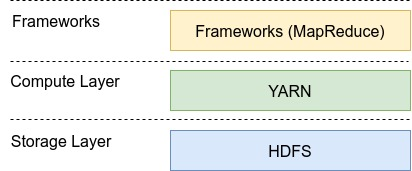
\includegraphics{images/HadoopHighLevelArch.jpeg}}
\caption{High Level Overview of Hadoop Architecture}
\label{highlevelarch}
\end{center}
\end{figure*}

\subsection{HDFS}
\emph{HDFS} is a distributed file system, designed handle large datasets. \emph{HDFS} embraces the idea that a write-once read-many data processing pattern is the most efficient. Typically within Hadoop an analysis of a dataset would use the whole of, or most of, the dataset so for \emph{HDFS} the read time of the entire dataset is more important than the latency of reading the first item in the dataset. 

\emph{HDFS} 

\subsection{YARN}


\subsection{MapReduce}
The MapReduce paper \cite{mapreduce} introduced a programming model for data generation and data processing. The model defines a computation which takes a set of key/value pairs as input and produces a set of key/value pairs as output.
This computation is composed of two different functions, \emph{Map} and \emph{Reduce}. \emph{Map} takes a key value pair as input and produces a set of \emph{intermediate} key/value pairs. These inermediate key/value pairs are processed by the \emph{MapReduce} library, which groups all values associated with each key and sends them to the \emph{Reduce} function. \emph{Reduce} takes the key and its set of values and produces zero or more outputs, depending on what the writer of the \emph{Reduce} function wanted to learn from the data.

Withing Hadoop, \emph{MapReduce} is a framework implementing the above programming model. It abstracts job resource management from writers of \emph{MapReduce} applications, calling the YARN API internally to have it schedule and manage \emph{MapReduce} jobs. Within this framework the unit of work is called a \emph{Job}. Hadoop executes a \emph{Job} 

\section{Conclusion}
The conclusion goes here.


\begin{thebibliography}{1}
\bibitem{mapreduce}
Jeffrey Dean and Sanjay Ghemawat, \emph{MapReduce: Simplified Data Processing on Large Clusters}, December, 2004.

\bibitem{gfs}
Sanjay Ghemawat, Howard Gobioff, and Shun-Tak Leung, \emph{The Google File System}, October, 2003.

\end{thebibliography}

\end{document}


